
\chapter{Neurónové siete}\label{chap:neuralnet}

Keďže \textit{umelé neurónové siete} sú významnou časťou tejto práce, venujeme im samostatnú kapitolu. Popíšeme čo sú neurónové siete, ako fungujú a základné typy neurónových sietí, ktoré používame v aplikácií.
\bigskip

\section{Jednoduchý spojitý perceprtón}

\begin{figure}[hp]
  \begin{center}
    \begin{subfigure}[b]{0.6\textwidth}
      \centering
      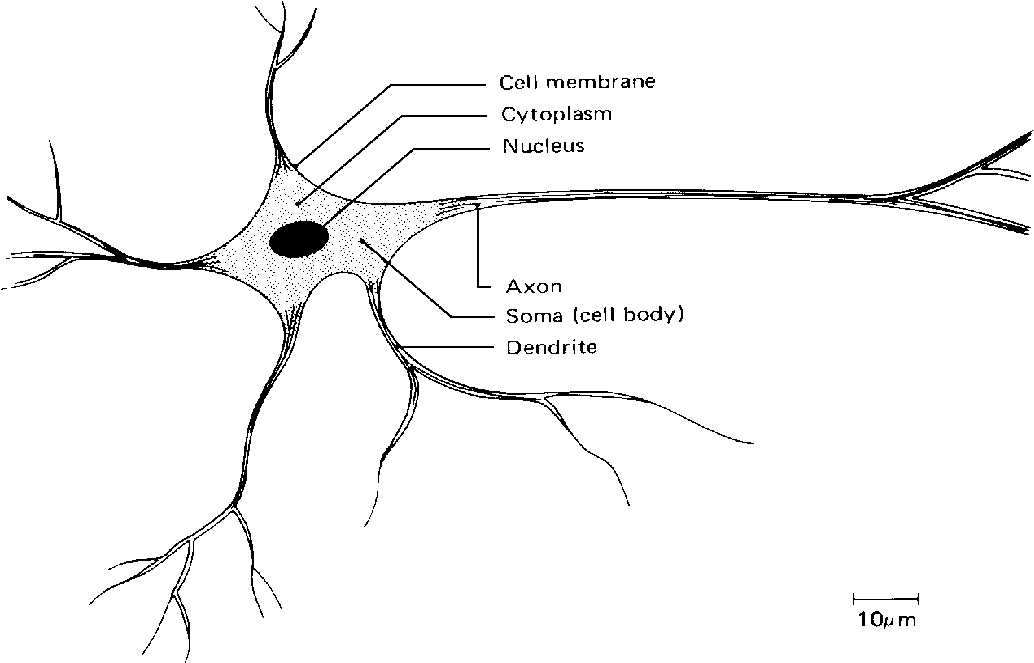
\includegraphics[width=\textwidth]{images/bio_neuron}
      \caption{Prírodný neurón}
      \label{fig:bio_neuron}
    \end{subfigure}
    \begin{subfigure}[b]{0.3\textwidth}
      \centering
 	  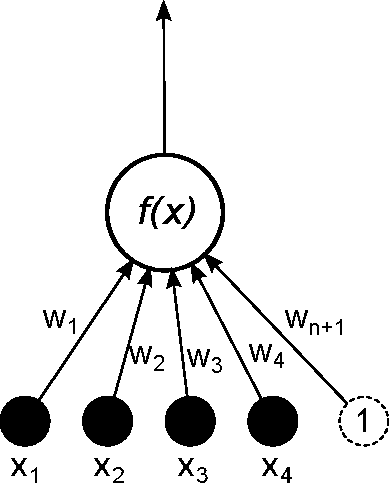
\includegraphics[width=\textwidth]{images/neuron}
 	  \caption{Umelý neurón}
 	    \label{fig:neuron}
    \end{subfigure}
  \end{center}%  
  \caption{Prírodný vs. umelý neurón}
\end{figure}

Jednoduchý perceptrón je inšpirovaný nervovou bunkou - neurónom. Vstupy umelého neurónu zodpovedajú \textit{dendridom}, výstup zodpovedá \textit{axónu}. 
Transformáciu vstupu na výstup zabezpečuje aktivačná funkcia.

Keď si neurón predstavíme ako orientovaný graf (Obr. \ref{fig:neuron}), za vrcholy položíme, vstupy, výstup a ,,telo" neurónu, vzniknú nám 2 typy hrán.
\begin{enumerate}
\item Synaptické -- vstup $\rightarrow$ neurón -- lineárna input-output väzba, kde pôvodný signál $x_i$ prenásobíme váhou synapsy $w_i$ a tým dostaneme výsledný signál $x_i'$.

\item Aktivačné -- neurón $\rightarrow$ výstup -- nelineárna input-output väzba, kde $y$ dostaneme dosadením $\sum x_i'$ do aktivačnej funkcie.
\end{enumerate}

K vstupom treba pridať ešte jeden vstup -- \textit{bias} -- ktorý má vždy hodnotu 1. Jeho význam je pri vstupe so samými nulami, pretože vtedy hodnoty na synapsách ostanú nezmenené a perceptrón by sa tento vzor nevedel naučiť.

Nech $n$ je počet vstupov a  $f$ je aktivačná funkcia. Výsledný signál $y$ dostaneme takto:

$$y= f\left(\sum_{i=1}^{n+1} w_i x_i \right)\qquad x_{n+1}=1$$\medskip

Aktivačnou funkciou spojitého je sigmoida: 

$$f(x) = \frac{1}{1+e^{-x}}$$\medskip
%Sigmoida bola vybratá preto, lebo spĺňa vlastnosti, ktoré má mať aktivačná funkcia.

Z matematického hľadiska robí takýto perceptrón zobrazenie $\mathbb{R}^n\rightarrow (0,1)$.

\section{Vrstva neurónovej siete}

Niekoľko perceptrónov vieme spojiť do jednej vrstvy. Získame tým vačší rozmer výstupu a teda môžeme vstupy klasifikovať do viacerých tried. Hodí sa to aj pri použití vo viacvrstvových sieťach.

Neuróny vo vrstve nie sú nijako pospájané a každý teda operuje nezávisle, takže z praktického hľadiska je to skupina neurónov pracujúcich nad tým istým vstupom.

Vrstva robí zobrazenie $\mathbb{R}^n\rightarrow (0,1)^m$, kde $n$ je rozmer vstupu a $m$ je počet neurónov vo vrstve.

\section{Viacvrstvová dopredná neurónová sieť}

\begin{figure}[htbp]
  \begin{center}
    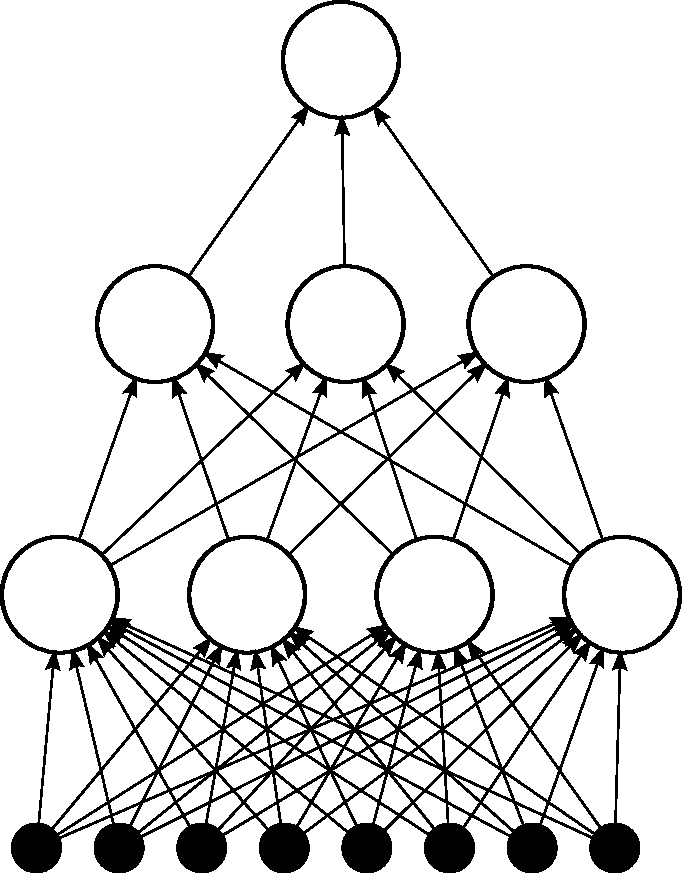
\includegraphics[width=0.3\textwidth]{images/ffnn}
  \end{center}
  \caption{Dopredná neurónová sieť}
  \label{fig:ffnn}
\end{figure}

Viacvrstvová neurónová sieť vznikne spojením niekoľkých vrstiev. Nižšia vrstva tvorí vstup pre vyššiu (obr. \ref{fig:ffnn}). Pôvodný vstup je vstupom pre najnižšiu vrstvu.

Viacvrstvová sieť umožňuje riešiť problémy, ktoré jedna vrstva riešiť nedokáže. Jedným z nich je napríklad funkcia xor \cite[s. 197]{haykin1999neural}. Vo všeobecnosti sa viacvrstvová sieť dokáže naučiť aj súvislosti medzi vstupmi.

Viacvrstvové neuónové siete sa trénujeme algoritmom backpropagation\footnote{algoritmus spätného šírenia chyby} \cite{haykin1999neural,dominika2011neural}.

\section{Rekurentná neurónová sieť}

V predchádzajúcich podkapitolách sme sa zaoberali doprednými sieťami (feedforward), v ktorých sa informácia šírila len smerom od vstupov k výstupu. V rekurentných sieťach máme navyše rekurentné spojenia, cez ktoré sa informácia prenáša v čase. Informácia z jednotlivých neurónov môže byť v ďalšom kroku použitá ako vstupná informácia pre neuróny.

\begin{figure}[htbp]
  \begin{center}
    \includegraphics[width=0.15\textwidth]{images/recneuron}
  \end{center}
  \caption{Rekurentný neurón}
  \label{fig:recurentneuron}
\end{figure}

Existuje veľké množstvo architektúr neurónových sietí, niektoré môžete nájsť v \cite[s. 755]{haykin1999neural}. My sme si vybrali oveľa jednoduchší model. Namiesto jednoduchých spojitých perceptrónov použijeme rekurentné neuróny (obr. \ref{fig:recurentneuron}).

Rekurentný neurón obsahuje navyše spätnú väzbu. Spätná väzba sa tvári ako ďalší vstup a obsahuje posledný \textbf{updatenutý} výstup toho istého neurónu. Po aktivácii neurónu môžeme updatnuť poslednú aktivačnú hodnotu. Ak to neurobíme, hodnota ostane taká, ako bola predtým. Neurón môžeme aj resetnúť, vtedy sa hodnota vynuluje.

Našu jednoduchú rekurentnú neurónovú sieť trénujeme tiež algoritmom backpropagation s tým, že sieti predkladáme postupnosti - vždy v tom istom poradí. Pri kladnej odozve updatujeme rekurentný vstup, ináč nie. Po každej postupnosti zresetujeme rekurentný vstup na 0.

%TODO vysvetlit? 

%\section{Algoritmus backpropagation (spätného šírenia chyby)}

%Algoritmus funguje v 2 fázach. V prvej fáze sa klasickým spôsobom vypočíta výstup a k nemu prislúchajúca chyba.

%V druhej fáze sa táto chyba spätne aplikuje na nižšie vrstvy, pričom je prenásobená príslušnou váhou -- t.j. ak máme neurón $y_i$ s chybou $e_i$ a $x_j$ je neurón, ktorý je $j$-tym vstupom neurónu $y_i$, tak ku chybe neurónu sa pripočíta $e_i w_{ij}$.

